\section{Introduction}
\paragraph{}Afin de réaliser le simulateur de réseau efficacement, nous avons commencé par
découper le projet en un ensemble de tâches (\textit{work packages}). Nous avons
attribué chaque ensemble de tâches à un responsable de \textit{work packages}.
Ces ensembles de tâches seront décrits dans une première partie.
\paragraph{}Pour représenter un réseau et effectuer des opérations sur celui-ci,
nous avons implémenté une structure \textit{graphe} avec des fonctions associées qui
seront décrites dans une deuxième partie.
\paragraph{}Puis, dans le but de réaliser ce réseau, deux types d'entités sont utilisées : le contrôleur et les routeurs. Le fonctionnement du contrôleur ainsi que
les choix de développement associés seront abordés dans une troisième partie.
\paragraph{}Dans une dernière partie seront abordés les choix de développement
concernant les routeurs.
\section{Gestion du projet}
\paragraph{}Afin de mener le projet à son terme, il nous a été nécessaire de segmenter les tâches. Pour ce faire, nous avons créé des ensembles de tâches
(\textit{work packages}) auxquels nous avons attribué des chefs de projets. Tous les
membres du groupe sont contributeurs sur tous les \textit{work packages}, conséquence du faible nombre de personnes au sein du groupe.
Les \textit{works packages} sont au nombre de quatre :
\newline
\begin{itemize}
\item Work package 1 :
    \begin{itemize}
	\item Gestion du projet
	\item Responsable : Arnaud Duforat 
    \end{itemize}
\vspace{1em}
\item Work package 2 :
    \begin{itemize}
	\item Contrôleur
	\item Responsable : Benjamin Bougot
    \end{itemize}
\vspace{1em}
\item Work package 3 :
    \begin{itemize}
	\item Routeur
	\item Responsable : Abderrahman Bentaleb
    \end{itemize}
\vspace{1em}
\item Work package 4 :
    \begin{itemize}
	\item Recette
	\item Responsable : Youssef Belbachir
    \end{itemize}
\end{itemize}
\paragraph{}A chaque \textit{work packages} est associé un certains nombre de tâches, dont la durée de réalisation a été estimée pour chacune d'entre elles et reportée sur un diagramme de Gantt. Cette gestion nous a permis de nous organiser plus efficacement dans la réalisation des objectifs majeurs du projet.
\newpage
    Les tâches de ces \textit{work packages} sont :
\begin{itemize}
\item WP1 :
    \begin{itemize}
	\item Analyse du sujet + répartition des tâches
	\item Création des \textit{work packages}
	\item Création d'un diagramme de Gantt
    \end{itemize}
\vspace{1em}
\item WP2 :
    \begin{itemize}
	\item Mise en place de la structure des graphes du contrôleur en C
	\item Ecriture du \textit{parser} des fichiers de configuration du contrôleur en C
	\item Mise en place de la communication client - serveur par \textit{sockets} en C
	\item Tests unitaires
    \end{itemize}
\vspace{1em}
\item WP3 :
    \begin{itemize}
	\item Mise en place de la classe du routeur en Java
	\item Mise en place de la communication client - serveur par \textit{sockets} en Java
	\item Gestion des \textit{threads} du routeur dans la classe \textit{RouterThread} en Java
	\item Gestion de ce qui est tapé sur l'entrée standard avec la classe \textit{Commande} en Java
	\item Ecriture du \textit{parser} des fichiers de configuration des routeurs en Java
	\item Tests unitaires
    \end{itemize}
\vspace{1em}
\item WP4 :
    \begin{itemize}
	\item Tests d'intégration
	\item Rédaction du rapport intermédiaire
	\item Rédaction du rapport final
    \end{itemize}
\end{itemize}
\paragraph{}Le projet se déroule selon le planning suivant :
\vspace{1em}
    \begin{figure}[!h]
	\begin{center}
	    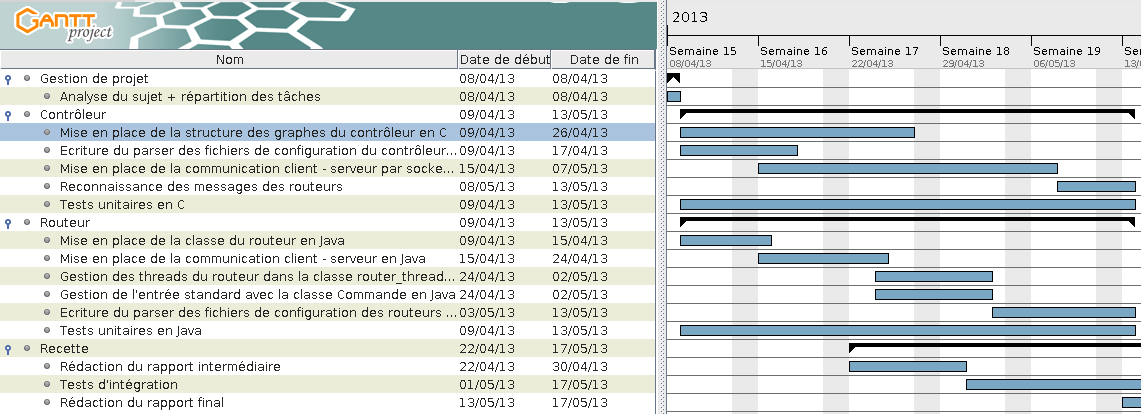
\includegraphics[scale=0.45]{gantt.png}
	\end{center}
	\caption{Diagramme de Gantt}
    \end{figure}
\newpage
\section{Graphe}
\paragraph{}Afin de respecter notre choix d'implémentation du contrôleur en langage C, nous avons également choisi ce langage pour réaliser le graphe. Nous avons décidé de représenter ce graphe sous forme d'une liste de successeurs, modélisée sous
forme d'un tableau de pointeurs structure \textit{noeud} représentant la liste
des noeuds du graphe. La structure \textit{noeud} contient un tableau de
pointeurs de structure \textit{noeud} qui représente la liste des noeuds voisins.
\\
\newline Les deux structures sont détaillées comme suit : 
\\
Structure graphe :
\begin{itemize}	
\item \textbf{nombre\_Noeud} : un entier représentant le nombre de noeuds du graphe.
\item \textbf{liste\_noeud}  : un tableau de pointeurs de structure \textit{noeud}, contenant les noeuds du graphe.
\end{itemize}
\vspace{1em}
Structure noeud :
\begin{itemize}
\item \textbf{label}   		: une chaîne de caractères contenant le label du noeud.
\item \textbf{id}    	     	: un entier pour identifier le noeud, il correspond à son indice dans le tableau des noeuds du graphe.
\item \textbf{nombre\_Voisin} : un entier représentant le nombre de voisins du noeud.
\item \textbf{cout}          : si le noeud est un successeur, il représente le coût associé, sinon c'est 0 par défaut.
\item \textbf{voisin}        : un tableau de pointeurs de structure \textit{noeud}, contenant la liste des voisins de chaque noeud.
\end{itemize}

\vspace{1em}
\noindent{}
Pour permettre au contrôleur de manipuler le graphe, nous avons
implémenté les fonctions suivantes :

\begin{itemize}
\item \textbf{void ajouter\_Noeud (struct graph* graph, char* label)} : permet de créer un noeud de nom label, et de le rajouter dans le graphe.

\item \textbf{void ajouter\_Lien ( struct graph* graph, char* label1, char* label2, int cout)} : permet de rajouter le noeud de label1 comme successeur du noeud label2 et vis versa, avec ajout du coût de la liaison. 

\item  \textbf{void supprimer\_Lien (struct graph* graph, char*label1, char*label2)} : supprime le noeud label1 de la liste des voisins du noeud label2 et vis versa.
 
\item \textbf{void deconnecter\_Routeur(struct graph* graph, char*label)} : supprime la liste des voisins du noeud label, et le supprime de la liste des voisins des autres noeuds.

\item \textbf{void modifier\_cout(struct graph* graph, char*label1, char*label2, int cout)} : met à jour le coût entre le noeud label1 et le noeud label2.
\item \textbf{void show\_Topology(struct graph* graph)} : affiche la topologie du réseau sur la sortie standard. 
\item \textbf{void sauvegarder\_Topology(struct graph* graph, char* nom\_fichier)} : sauvegarde la topologie dans un fichier dont on spécifie le nom.
\end{itemize}


\newpage
\section{Contrôleur}

\subsection{Choix du langage de programmation}
\paragraph{}Afin de réaliser le contrôleur, notre choix s'est naturellement porté
vers le langage C. En effet, ses possibilités d'optimisation, sa légèreté et sa rapidité nous permettent de concevoir efficacement les principales fonctionnalités du contrôleur. Parmi ses fonctions, nous pouvons mentionner le calcul des tables de routage des routeurs, la gestion des connexions avec plusieurs routeurs et la réalisation de nombreuses autres opérations plus élémentaires.
\paragraph{}De plus, une autre fonction importante du contrôleur est d'offrir la possibilité de récupérer la topologie du réseau formé par le contrôleur et les routeurs. Dans ce projet, la topologie du réseau peut être décrite à l'aide de fichiers de données représentant des graphes, au format \textit{.gv}. Afin de réaliser cet objectif, nous nous sommes intéressés au logiciel de visualisation de graphe, \textit{GraphViz}. Ce logiciel fournit une bibliothèque, \textit{cgraph}, permettant de lire des graphes au format \textit{.gv}. Cette bibliothèque est disponible par le biais du langage C, ce qui justifie ainsi le choix de ce langage.

\subsection{Structure utilisée par le contrôleur}
\paragraph{}Nous avons créé une structure Client, qui contient le socket du routeur, le nom du routeur, une liste de ses voisins, le temps de sa dernière connexion (la dernière fois qu'il s'est connecté), son numéro de port et son adresse IP. Cette structure a été gardée a part mais on aurait pu également développer une méthode pour que les noeuds de la topologie contiennent directement ces informations. De cette façon, on aurait pu optimiser les accès en les diminuant encore. En réalité, les accès aux informations d'un client donné sont linéaires sur le nombre de clients. Ainsi, dans le cas actuel, la complexité pour récupérer n'importe quelle information est \textit{2 * Nombre de clients}, soit O(2n) avec n, le nombre de clients pour un accès en lecture. Si on avait fait en sorte que les noeuds du graphe reçoivent directement les informations du routeur, on aurait une complexité de O(n). Compte tenu du temps qui nous était imparti, nous avons jugé bon que ce n'était pas prioritaire mais qu'il serait envisageable de développer à partir de notre code.

\subsection{\textit{Parser} du fichier de configuration du contrôleur}
\paragraph{}Afin de s'initialiser correctement, la première opération que doit faire le
contrôleur est de lire un fichier de configuration contenant le numéro
du port TCP d'écoute, et de lire le temps entre deux requêtes effectuées par les
routeurs au contrôleur au-delà duquel le routeur est retiré du réseau
(\textit{timeout}).
\paragraph{}Pour cela, nous avons créé  en langage C un \textit{parser} de fichier de configuration possédant une structure \textit{options} contenant les différents paramètres que l'on souhaite sauvegarder. Le \textit{parser} contient une fonction \textit{parse()} prenant en paramètre le chemin du fichier à ouvrir et qui permet de charger les données dans la structure \textit{options}.
\paragraph{}Par ailleurs, il nous a semblé important d'intégrer certaines fonctionnalités supplémentaires, telles que la gestion de la présence de commentaires,
de lignes vides ou contenant autant d'espaces que l'on veut. Ainsi, il est possible de
mettre les options dans l'ordre de son choix dans le fichier de
configuration. Les valeurs attribuées aux options sont vérifiées, en
particulier les entiers et les adresses IP. La structure du \textit{parser} peut également être facilement modifiée afin d'ajouter de nouvelles options et des vérifications
associées.

\subsection{\textit{Parser} du fichier de graphe}
\paragraph{}Le \textit{parser} du fichier de graphe permet de lire des fichiers de graphe au format \textit{.gv} et affiche des images au format \textit{png} permettant de visualiser la topologie du réseau.
\paragraph{}Les informations recueillies sont ensuite stockées dans une
structure \textit{node} contenant le label d'un noeud (par exemple \textit{N1}), le code du noeud dans le fichier de graphe (par exemple \textit{n1}), ses voisins et le
coût de chacune des liaisons avec les voisins. Ces noeuds sont alors
stockés dans une structure \textit{nodes\_container} qui est en fait un tableau
dynamique de structures \textit{node}.
\paragraph{}Une fonction \textit{readFile()} prenant en paramètre le fichier
permet de remplir ces structures. 
\subsection{Commandes}
\paragraph{}Nous avons implémenté le totalité des commandes permettant d'interagir avec la topologie. Les commandes suivantes ont été réalisées :
	    \begin{itemize}
		    \item \textbf{load}    : charge la topologie décrite dans un fichier texte (\textit{.txt}).
		    \item \textbf{show}     : affiche la topologie chargée.
		    \item \textbf{add} : ajoute un lien entre deux noeuds en spécifiant le coût associé.
		    \item \textbf{del}  : supprime un lien entre deux routeurs.
		    \item \textbf{disconnect} : déconnecte un routeur du réseau en supprimant tous ses liens.
\item \textbf{update} : modifie le coût d'un lien dans le réseau.
\item \textbf{save} : sauvegarde la topologie actuelle dans un fichier.
	    \end{itemize}
\subsection{Commandes envoyées par les routeurs au contrôleur}
\paragraph{}Nous avons implémenté la gestion des commandes reçues par le contrôleur, provenant des routeurs. Les commandes suivantes ont été réalisées :
	    \begin{itemize}
		    \item \textbf{log in as .. port ..}    : connexion d'un routeur au contrôleur en spécifiant un identifiant et un numéro de port. Si l'identifiant n'est pas mentionné ou qu'il n'existe pas dans la topologie, le contrôleur peut lui envoyer un identifiant libre.
		    \item \textbf{lot out}     : déconnexion du routeur au contrôleur.
\item \textbf{poll} : demande la topologie au contrôleur. Le principe consiste à regarder les noeuds voisins du routeur appelant. Dans la topologie, chaque noeud du graphe contient un booléen \textit{activated}, donc il est possible de connaître les noeuds réellement actifs et ceux qui ne sont pas actifs, c'est à dire ne correspondant pas encore à un routeur. Il est donc possible de ne retourner que les voisins directs. La complexité est ainsi minimale (linéaire en nombre de voisins).
	    \end{itemize}
\subsection{Sockets en C}
\paragraph{}Nous avons réalisé un serveur (contrôleur) permettant la communication
entre des clients (routeurs) et pouvant lui-même communiquer avec les
routeurs. Pour cela, le contrôleur ouvre autant de \textit{sockets} que de routeurs
et effectue une commande \textit{select} sur ces \textit{sockets} pour attendre les changements d'état et agir en conséquence. Ainsi, la communication est pseudo-asynchrone,
garantissant ainsi des performances correctes. De plus, on n'utilise qu'un
seul port pour toutes les connexions et on n'a pas besoin de créer un
\textit{thread} par connexion.
\paragraph{}Concernant le contrôleur, le routeur est représenté par une structure
\textit{Client} contenant le \textit{socket} utilisé par le routeur et son nom permettant de l'identifier (\textit{N1} par exemple).
\newpage
Nous avons réalisé l'implémentation des opérations suivantes : 
\begin{itemize}
\item Création de connexion et initialisation, avec identifiant spécifié ou non (attribution d'un identifiant libre dans ce cas).
\item Terminaison de connexion.
\item Lecture des informations envoyées par les routeurs.
\item Écriture vers les routeurs.
\item Envoie de messages à tous les routeurs présents.
\item Suppression d'un routeur ou de tous les routeurs.
\item Demande de la topologie d'un noeud.
\end{itemize}

\section{Routeurs}
\paragraph{}Afin de réaliser le routeur, le choix du langage de programmation s'est porté sur le langage Java. En effet, nous avons décidé d'utiliser un langage qui était familier au plus grand nombre d'entre nous, afin de pouvoir contribuer tous ensemble à sa réalisation. De plus, le choix d'un langage orienté objet était justifié par le fait que nous avions à traiter un grand nombre d'entités (ici des routeurs), d'où la nécessité d'avoir une approche modulaire lors de leur conception. Enfin, la réalisation de \textit{parser} et la gestion des sockets sont particulièrement simples et efficaces en Java. 

\subsection{Architecture}
\begin{itemize}
\item \textbf{Router} : C'est la classe principale de la partie routeur. \\
	Elle contient toutes les méthodes de bases (ajouter un routeur,
	supprimer...). \\
	    Initialement, elle ouvre un socket, lance le thread Commandes
	    et un thread RouterThread pour chacun des routeurs qui se
	    connectent sur sa propre socket.
\item \textbf{RouterThread} : cette classe est un thread lancé pour chaque
	    routeur voisin. \\
	    Cette classe ne fait qu'écouter le canal entre
	    deux routeurs connectés, et peut écrire ce qu'elle reçoit sur la
	    sortie standard. Avant de commencer l'écoute
	    du canal, le routeur attend la réception de l'identifiant du
	    routeur.
\item \textbf{Commandes} : Cette classe gère tout ce qui est tapé sur l'entrée
	    standard. Chaque commande tapée est soit validée soit rejetée.
	    La liste des commandes que l'on a pu implémenter est :
	    \begin{itemize}
		    \item \textbf{total}    : donne le nombre des routeurs connectés.
		    \item \textbf{quit}     : arrête le routeur.
		    \item \textbf{add port} : ajoute une liste de voisin à la main.
		    \item \textbf{connect}  : se connecte à tous les voisins ajoutés,
			et envoie le message "link id ID".
		    \item \textbf{message ID "MESSAGE"} : envoie "MESSAGE" au routeur
			d'identifiant ID.
\item \textbf{ControllerThread} : Il s'agit d'une classe qui, périodiquement, demande la liste des voisins à ses contrôleurs.
\item \textbf{PeriodicVector} : Il s'agit d'une classe qui, périodiquement, envoie le vecteur distance à ses voisins. On a prévu de s'en servir pour la gestion des tables de routage.
\item \textbf{ParsePing et ParsePaquet} : Il s'agit de classes qui lisent les données envoyées au routeur.
	    \end{itemize}
\item \textbf{RouterInfo} : dans la classe, nous avons une liste de cette
	    classe dont on enregistre les routeurs voisins et toutes les
	    informations dont nous aurons besoin par la suite.
\end{itemize}

\subsection{Justification de l'architecture}
	\paragraph{}Au départ, nous avions essayé de créer un thread qui se chargeait de la
	lecture et de l'écriture en même temps pour chaque connexion. Le
	problème que l'on a rencontré est que ces deux actions sont bloquantes. De plus, nous avions également un problème d'accès concurrent aux informations
	tapées sur le clavier puisque la lecture se faisait sur l'entrée
	standard.

	\paragraph{}Une deuxième solution était de créer un thread pour la lecture
	et un autre pour l'écriture. Cependant, cela ne corrige pas le
	problème de l'accès concurrent et le nombre de thread double, ce qui
	limite le nombre de routeurs dans notre réseau virtuel.

	\paragraph{}La troisième solution, que l'on a finalement décidé d'utiliser, 
	est de créer un seul thread pour chaque connexion qui ne se chargera
	que de la lecture, puis on a ajouté un thread (Commandes) qui se charge
	de la lecture depuis l'entrée standard. Cette classe analyse ce que
	l'utilisateur tape ou ce que les autres routeurs envoient. Supposons
	que l'utilisateur veut envoyer un message à un autre routeur (message
	N3 "le message"), le thread commande va extraire l'identifiant, puis
	va chercher dans la liste des voisins le routeur avec le bon
	identifiant et va finalement écrire dans sa sortie sans avoir besoin
	d'un thread d'écriture.

	    Avec cette dernière solution on a pu :
\begin{itemize}
\item régler le problème de l'accès concurrent sur l'entrée standard.
\item diminuer le nombre de threads créés.
\item supprimer les actions bloquantes.
\end{itemize}

\subsection{Fonctionnalités implémentées}

\subsubsection{Communication entre routeurs et contrôleur}
Nous avons réussi à faire communiquer correctement le routeur et le contrôleur en respectant le protocole. Nous avons implémenté la liste de fonctionnalités ci-dessous : 
\begin{itemize}
\item \textbf{Initialisation} : le contrôleur attribue au routeur un identifiant.
\item \textbf{Topologie} : le routeur envoie périodiquement la commande poll* au contrôleur. Il reçoit la liste de ses voisins. Si le routeur reçoit la liste vide, il se déconnecte de ses voisins.
\item \textbf{Finalisation} : un routeur est supprimé s'il le demande de manière explicite sous forme d'un log out, ou sinon, s'il ne communique plus avec le contrôleur au bout d'un certain temps.

\end{itemize}


\subsubsection{Communication entre routeurs}

Le protocole de communication entre routeurs a été entièrement développé. Nous avons réussi à implémenter les fonctionnalités suivantes : 

\begin{itemize}
\item \textbf{Connexion} : le routeur parcourt la liste de ses voisins et établi une connexion TCP/IP avec eux.

\item \textbf{Liste des vecteurs distance} : chaque routeur parcours sa liste de voisins et construit un vecteur qu'il envoie à tous ses voisins.

\item \textbf{Paquets} : le routeur construit un paquet à chaque fois qu'il veut envoyer un message. Ce paquet contient le numéro de séquence, son adresse IP source, l'adresse IP destination, la valeur du TTL, et la chaine de caractères à transmettre. Au tout début de la communication, le routeur ouvre une connexion TCP/IP avec le contrôleur et reçoit la liste de ses voisins. Quand l'utilisateur tape la commande \textit{"message id .."}, le routeur cherche le voisin avec l'\textit{id} correspondant, sinon il envoie le message d'erreur: \textit{"Unknown Destination"}. 

\item \textbf{Ping} : le routeur envoie la ligne de commande \textit{ping} contenant le numéro de séquence, l'\textit{id} de la source, l'\textit{id} du routeur de destination, et la valeur de TTL. Cette valeur se décrémente à chaque fois qu'elle passe par un routeur intermédiaire. Le routeur source reçoit un \textit{pong} avec un \textit{ttlzero} si le paquet n'est pas acheminé.

\item \textbf{TraceRoute} : le routeur envoie la route empruntée par les paquets jusqu'à arriver à une certaine destination. Cette fonctionnalité a été implémentée mais nous n'avons pas eu le temps de la tester complètement.

\end{itemize}
\newpage
\section{Problèmes rencontrés}
\paragraph{}Le problème principal rencontré était plus lié à la gestion du temps qu'à des problèmes techniques. En effet, ce fut l'élaboration des communications entre les routeurs  et le contrôleur qui a demandé une grande réflexion sur l'architecture, ce qui a eu un impact non négligeable sur le temps accordé à cette tâche. 
\section{Limites}
\paragraph{}Nous n'avons pas eu le temps d'implémenter la gestion des tables de routage. 
\section{Tests unitaires}
\subsection{Contrôleur}
\paragraph{}Nous avons réalisé un certains nombre de tests, validant les différentes fonctionnalités que l'on a pu implémenter.
\begin{itemize}
\item \textbf{Le test de chargement de fichiers de configuration} : Nous avons réalisé différents tests en créant plusieurs fichiers de tests : Des fichiers valides qui contiennent une syntaxe gérée par le contrôleur, des espaces entre les commandes, des commentaires et une indépendance vis à vis de l'ordre concernant les paramètres. Puis nous avons écrits des fichiers invalides contenant des entrées incorrectes (par exemple, la présence de texte dans l'entrée du port d'un contrôleur, des numéros de ports négatifs ou dépassant les bornes (0 - 65535). Ces fichiers sont testés grâce au fichier \textit{test\_cfgparser.c}.
\item \textbf{Le test de chargement des graphes décrivant une topologie} : Ce test permet de vérifier que le chargement d'un fichier de graphe est correct. Ce test est accessible via le fichier \textit{test\_parser.c}.
\item \textbf{Le test de commandes entrées au clavier} : Nous utilisons la fonction \textit{analyse\_cmd} qui analyse habituellement ce qui est entré au clavier afin de comparer avec ce qui est attendu. Ce test est accessible via le fichier \textit{test\_commandParser.c}. 
\item \textbf{Le test de la structure représentant la topologie} : Il s'agit d'une procédure consistant en un enchainement d'ajouts et de suppression de noeuds et d'arêtes puis qui vérifie si le résultat est correct et l'affiche. Ce test est accessible via le fichier \textit{graph\_test.c}.
\end{itemize}
\section{Conclusion}
\paragraph{}Nous regrettons de ne pas avoir bénéficié de plus de temps pour réaliser ce projet. En effet, celui-ci a été très intéressant et nous a aidé à consolider nos connaissances en réseau et en programmation système en général. Il nous a permis de nous rendre compte du travail effectué par un routeur et des algorithmes de routage, par exemple lors de la réception d’un ping, ou d’un paquet. Le diagramme de Gantt a été correctement suivi dans sa globalité, bien que certaines tâches aient pris du retard (notamment l'implémentation des sockets).